%! suppress = TooLargeSection
\section{Coffee in society}
\label{sec:coffee-in-society} In recent years, coffee has gained more and more popularity,
cementing itself as one of the most widely consumed beverages~\cite{coffeeConsumptionStats}.
Along with a surge
in café openings, preparing coffee at home is now an activity enjoyed by more
and more people, with the average consumer being more discerning and critical than
ever.

The development of the coffee industry is often described as a series of ''waves``.
The first ''wave`` made coffee an everyday staple, focusing on convenience and high
availability.
During the second wave, the idea of ''specialty`` coffee first entered
the consumer vocabulary, with creative recipes, flavours and textures being popularised
by emerging cafés and chains.
The third wave, starting around 1980 and lasting to
the present day saw a significant shift in consumer values, placing more importance on the natural characteristics
of the beans themselves than on complex recipes and additional flavours.
It is also during this time that coffee
processing and roasting were moved into focus, with the average consumer being more
and more likely to differentiate and prefer a certain flavour profile over others~\cite{coffeeWaves}.

It should also be noted that the preference in roast levels have also shifted as
the waves changed.
During the second wave, when additional flavours and textures
were the key focus of drinks, a darker roast was preferred, as espresso produced
with a darker roasted bean will have a more mellow, sweet taste, with little to no
acidity (though, a higher chance of bitterness if the coffee / water ratios are not
correct), and a thicker, heavier body.
With this style of preparation, an equal
ratio of water to ground coffee is used, yielding a smaller, more intense
espresso.

In contrast, a ''third-wave`` coffee preparation style values the acidity and floral
notes that can only be retained through a very light, gentle roasting process.
For
many modern coffee enthusiasts, the lightest possible roast level is the most
desirable.
While an under-roasted bean will taste unpleasant to a vast majority,
with grassy, vegetal notes, a roast level above ''medium`` is thought to mask
away the harder to retain flavour notes coming from either the coffee processing
method, its origin or both.
%As lighter roasted coffee is less soluble and
%therefore more difficult to extract, modern coffee establishments often use higher
%coffee to water ratios, with 1:3 or even 1:5 ratios used to brew espresso.
%Drinks
%brewed this way sacrifice a thicker body for clarity and brightness of flavour,
%exposing as much of the bean's flavour profile as possible.
With the coffee flavour
placed front-and-center, it is now more important than ever for coffee producers
to deliver the best possible quality of their product.

This shift of consumer patterns has placed a lot of importance on coffee
roasters and farmers, who are now held to a higher standard than ever before.
Even a small percentage of defects, whether in the green (unroasted) coffee or in
the final product, can ruin a brewed drink.
As environmental issues and quality control
at farms is often out of the roasters' control, it is therefore extremely important
that the roasters are able to detect defects on their side with as much precision
as possible.

The following section will discuss the challenges faced by coffee roasters and producers
as well as describe the ''state of the art`` of quality control in coffee production.

\section{Coffee production challenges}
\label{sec:coffee-production-challenges}
%\begin{wrapfigure}
%{r}{0.35\textwidth}
%	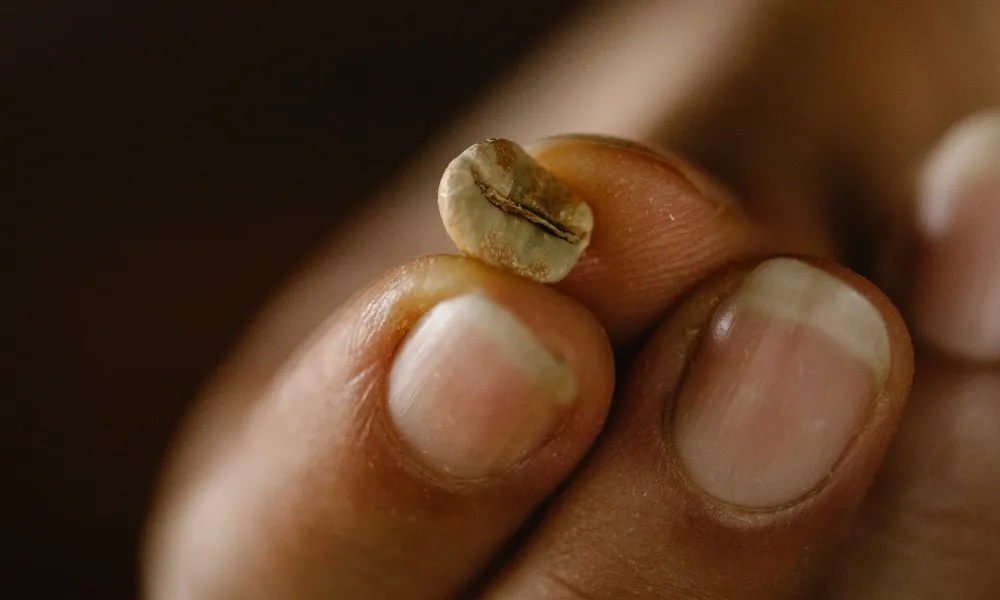
\includegraphics[width=0.35\textwidth]{figures/introduction/quaker-coffee-bean}
%	\caption*
%	{Source: \cite{quakerBeanImg}}
%	\caption{A ''quaker`` coffee bean.}
%	\label{fig:quakerBeanExample}
%	\vspace{-2em}
%\end{wrapfigure}
The worsening climate conditions,
rising consumer expectations and economic instability are just a few of the
challenges faced by the coffee roasting industry.
As many roasteries are quite small
businesses, addressing supply chain issues is often beyond their control, with roasters
having to perform secondary quality control to address the shortcomings of the previous
stages in the beans' journey.

Defective green coffee beans can seriously damage the flavour of the finished
product.
The most common defect occurs when the coffee cherry does not develop the
necessary sugar content due to being harvested before fully maturing or disease of
the plant: the beans within these cherries do not respond well to roasting, developing
an extremely unpleasant flavour which is typically compared to burnt paper, with
an astringent, drying sensation in the mouth~\cite{colourSorterImg}.
Such beans are commonly referred
to as ''quakers`` and, when roasted, can be identified by an uneven, spotty exterior caused by a lack of sugar caramelisation.
%as seen on figure \ref{fig:quakerBeanExample}.
%The spotty pattern develops due
%to the lack of sugar, preventing the bean from fully caramelising during roasting.
The unpleasant flavour brought along by such beans is extremely potent, with just
a few being able to ruin a large batch of otherwise acceptable product.

Apart from harming the taste of the roasters' products, such beans can also prevent
the roasters from achieving certain certifications or using certain marketing language.
The Specialty Coffee Association (SCA) is one of the most influential regulatory
bodies in the coffee industry.
The term ''specialty`` can only be used to describe
coffee when certain criteria are achieved: each batch of green coffee is roasted
and tasted, with the tasters awarding points for various aspects of the drink's flavours.
In order to achieve specialty status, the coffee has to earn over 80 points, as
well as being free from the previously mentioned defects~\cite{scaCuppingProtocol}.

As the ''specialty`` mark is often necessary for a roaster to stand out among
its competition and make itself known to coffee enthusiasts, quality control is one
of the most important tasks that a coffee roaster faces on a daily basis.

\section{State of the art in coffee quality control}
\label{sec:qc-state-of-the-art} Despite the previously described importance of quality
control, the automation options are surprisingly limited, requiring many medium-to-small
scale roasters to perform their quality control manually.
\begin{wrapfigure}
{r}{0.4\textwidth}
	\includegraphics[width=0.4\textwidth]{
		figures/introduction/colour-sorter-scale
	}
	\caption*
	{Source: \cite{colourSorterImg}}
	\caption{An industrial colour grader}
	\label{fig:colourSorterExample}
\end{wrapfigure}
While the knowledge
and expertise of many roasters allows them to perform this task relatively
easily, it still requires a significant amount of time and manual labour,
preventing the roasters from performing other tasks.
Furthermore, this approach
does not guarantee repeatable or even correct results, depending fully on the judgement
of the person performing it.
It should be noted that some commercial solutions are offered: industrial scale colour
graders can provide a high degree of accuracy and efficiency.
These machines use
image recognition to assign the beans one of several pre-determined categories,
using blasts of compressed air to remove defective beans as they fall through the
air.
These machines, however, are often a poor fit to all but the largest coffee
roasters due to several reasons:
\begin{itemize}
%	\item Prohibitive pricing, often tens of thousands of pounds
%		\begin{itemize}
%			\item With colour graders costing well into the tens of thousands of pounds,
%				purchasing one is a difficult to justify investment for most small
%				roasters.
%				Given the cost of specialty-grade green coffee, the roasters' profit
%				margins are usually quite narrow, therefore the value of such an
%				investment will become apparent only after an extremely long period of
%				time.
%				Additionally, these machines come with significant operating costs
%				which will be discussed further.
%		\end{itemize}

	\item Prohibitive pricing, large dimensions (as seen on figure~\ref{fig:colourSorterExample}), noise and high energy consumption
%		\begin{itemize}
%			\item Figure \ref{fig:colourSorterExample} shows a colour grader in use.
%				From the figure, the challenges brought along by these devices'
%				dimensions are clear: their large height, noise and energy consumption
%				often make them incompatible with the spaces occupied by many small
%				scale roasters.
%		\end{itemize}

	\item Usage of proprietary datasets, with little to no transparency on the sources of the data
%		\begin{itemize}
%			\item Most colour graders use some kind of image classification algorithm to
%				sort the beans.
%				While this allows for high classification speeds and
%				good accuracy, few manufacturers provide information on the dataset that
%				was used to develop the classifier.
%				While this is unlikely to pose an
%				issue with the most frequently consumed coffee varieties, rare coffee species
%				or beans that have undergone an unusual processing method may not fit into
%				the model used by such machines.
%				Therefore, these machines lack flexibility
%				and may not be suitable for roasters who often switch their beans or attempt
%				to experiment with roasting or processing techniques.
%		\end{itemize}

	\item Design that has large production lines in mind, requiring additional equipment such as air compressors, portioning and packaging machines, etc.
%		\begin{itemize}
%			\item As discussed above, most colour graders are aimed at production done
%				at a scale significantly exceeding that of most small-to-medium coffee
%				roasters.
%				Many colour graders are designed to be a part of an automated ``production
%				line'', with the beans being moved through chutes between the roaster, grader
%				and any further machinery, e.g. a portioning and packaging machine.
%				Given that many roasters roast in batches that are an order of magnitude
%				smaller than ones that can benefit from such machinery, colour graders simply
%				do not fit in their workflow.
%				Furthermore, even to achieve their basic functionality,
%				colour graders need an additional air compressor, further adding to the costs
%				associated with incorporating one into one's production.
%		\end{itemize}
\end{itemize}

\section{Research aims}
\label{sec:research-aims}
While colour graders are impractical for a significant
number of coffee roasters, their functionality would bring a significant benefit
at any level of production scale.
Furthermore, given the current trends in coffee
consumption and the pressure to deliver new products more often than ever,
proprietary datasets may not stay up to date with the variety of coffee beans available at
a given moment.

Therefore, this project aims to evaluate currently available image recognition algorithms
for recognizing roasted coffee defects and deliver a prototype which is:
\begin{enumerate}
	\item \label{itm:goal1} Cheap to train and operate

	\item \label{itm:goal2} Able to use custom datasets

	\item \label{itm:goal3} Able to adjust to new trends in coffee growing and processing

	\item \label{itm:goal4} Accurate and reliable
\end{enumerate}

It should be noted that this project is far from the first in identifying this problem:
the following section will contain a review of the state of the art as it applies to both
coffee quality control and image recognition in general.

A solution that achieves the above criteria could allow coffee roasters to have
deeper insights on their roasting technique, the quality of the green coffee they
purchase, as well as reduce the mental and physical workloads of quality control.

\section{Report structure}
\label{sec:report-structure}
In the following chapters, the following content will be covered: chapter~\ref{ch:litreview} will discuss the state of the art
in image classification and its past applications to similar problems, chapter~\ref{ch:methods} will outline the theoretical background
of the implementation decisions taken, chapter~\ref{ch:results} will provide a description of the resulting implementation and evaluate
its results, while chapter~\ref{ch:conclusion} will discuss the economical and ethical considerations of the work done as well as identify future
areas of development.